\documentclass[12pt,a4paper]{article}
\usepackage[utf8]{inputenc}
\usepackage{amsmath}
%\usepackage[brazilian]{babel}
\usepackage{breqn}
\usepackage{amsfonts}
\usepackage{amssymb}
\usepackage{graphicx}
\usepackage[margin=0.8in]{geometry}


\begin{document}
\title{\vspace{70mm}\Huge Experimento 02 - Pêndulo de Torção}
\author{ Giovani Garuffi\qquad\hfill
		\textit {RA: 155559}\protect\\
		João Baraldi\hfill
		\textit{RA: 158044}\protect\\
		Lauro Cruz\hfill
		\textit{RA: 156175}\protect\\
		Lucas Schanner\hfill
		\textit{RA: 156412}\protect\\
		Pedro Stringhini\hfill
		\textit {RA: 156983}								
		}
\maketitle
\newpage
\section{Resumo}


\section{Objetivos}
Calcular o módulo de Cisalhamento de um fio metálico, a partir do estudo da relação do periodo $(T)$ e comprimento do fio $(L)$ em um pêndulo de torção.


\section{Procedimento Experimental e Coleta de Dados}

\subsection{Materiais utilizados}
\begin{itemize}
	\item Pêndulo de torção com fio metálico
	\item Trena
	\item Paquímetro
	\item Micrômetro
	\item Photo-gate
	\item Cronômetro inteligente
\end{itemize}

\subsection{Procedimento}
O pêndulo foi montado usando-se um fio metálico tendo um cilindro de latão acoplado em sua ponta. Foram medidos o diâmetro do fio (com o micrômetro) e contabilizada a massa do cilindro (já previamente neles explicitada). Ao lado do da base do pêndulo, foi montado o photo-gate conectado a um cronômetro inteligente configurado no modo \emph{Pendulum}, para ser realizada a medição dos perídos de rotação. Para cada comprimento L do fio foram feitas 7 medições de período para fazer-se assim uma média aritmética. Todas as medições mencionadas foram registradas no relatório.  A montagem do experimento pode ser vista nas figuras 1 e 2.

\begin{figure}[!htbp]
	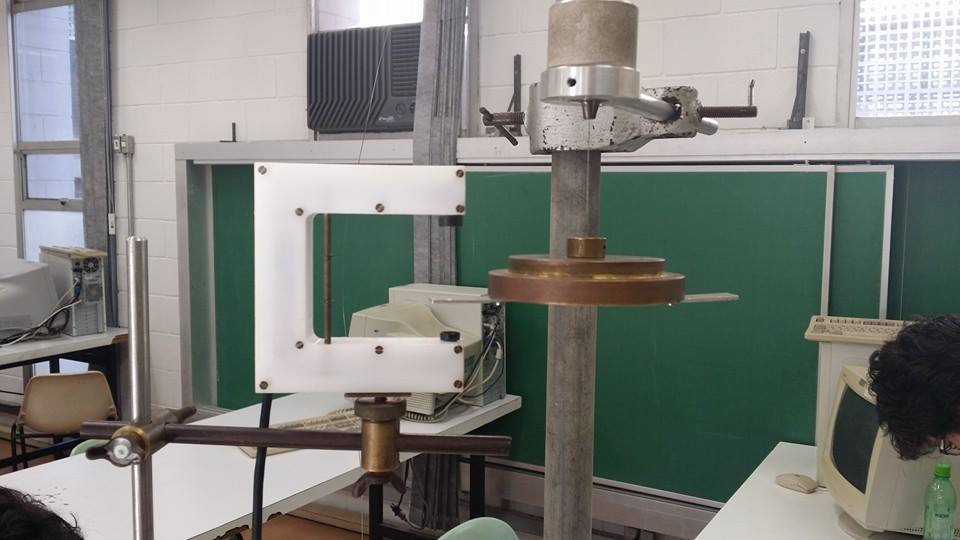
\includegraphics[scale=0.50]{03.jpg}
	\caption{Medição dos períodos}
	\label{fig:cilindro}
\end{figure}

\begin{figure}[!htbp]
	\centering
	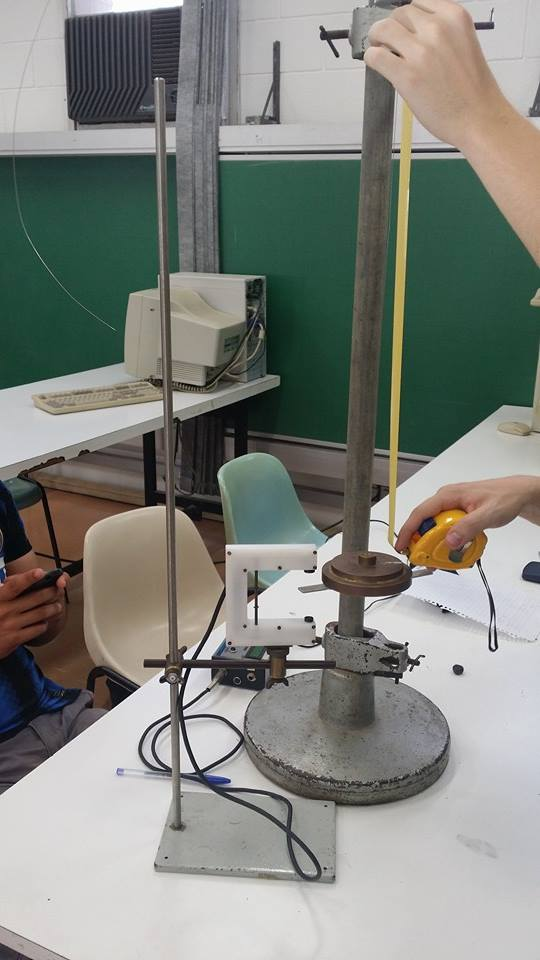
\includegraphics[scale=0.30]{01.jpg}
	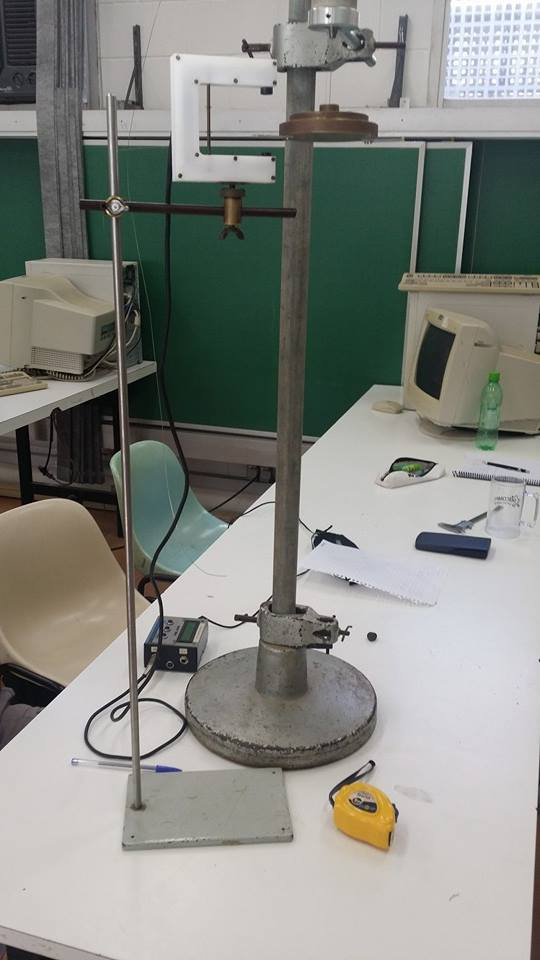
\includegraphics[scale=0.30]{02.jpg}
	\caption{Montagem do experimento}
\end{figure}

\subsection{Dados Obtidos}
O valor do diâmetro do fio é:
$$ d = (0.56 \pm 0.01) mm, $$
sendo $0.01 mm$ o erro intrumental do micrômetro.\\\\
A massa do conjunto de cilindros, previamente medida, é:
$$ M = (1198.2 \pm 0.1) g,$$
sendo $0.1 g$ o erro intrumental da balança usada.\\\\
Os valores dos períodos medidos $(T)$ para cada comprimento da linha $(L)$ podem ser encontrados na tabela 1.

\begin{table}[!htbp]
\def\arraystretch{1.3}
\caption{Peridos medidos $(T)$, relacionados ao comprimento do fio ($L$)} 
\label{Resultados}
\begin{tabular}{|l|ccccccc|r|}
\hline 
L $(m)$ & \multicolumn{7}{c|}{Medidas de Periodo $(s)$} & Periodo Médio $(s)$ \\ 
\hline 
0.540 & 5.7902 & 5.7958 & 5.7987 & 5.8002 & 5.7968 & 5.8066 & 5.7940 & $5.797 \pm 0.002$\\
\hline 
0.503 & 5.5987 & 5.6002 & 5.5993 & 5.5996 & 5.5959 & 5.5928 & 5.5928 &$ 5.597 \pm 0.001$\\
\hline 
0.415 & 5.1084 & 5.1099 & 5.1076 & 5.1058 & 5.1000 & 5.1072 & 5.1072 & $5.107 \pm 0.001$\\
\hline 
0.360 & 4.7782 & 4.7815 & 4.7706 & 4.7755 & 4.7722 & 4.7716 & 4.7689 & $4.774 \pm 0.002$\\
\hline 
0.298 & 4.3553 & 4.3612 & 4.3617 & 4.3604 & 4.3591 & 4.3578 & 4.3570 & $4.359 \pm 0.001$\\
\hline 
0.234 & 3.8980 & 3.8927 & 3.8898 & 3.8860 & 3.8833 & 3.8801 & 3.8766 & $3.887 \pm 0.003$\\
\hline 
0.155 & 3.2135 & 3.2136 & 3.2124 & 3.2184 & 3.2141 & 3.2164 & 3.2151 & $3.215 \pm 0.001$\\
\hline 
0.142 & 3.0867 & 3.0862 & 3.0898 & 3.0955 & 3.0933 & 3.0945 & 3.0242 & $3.081 \pm 0.009$\\
\hline 
0.088 & 2.5071 & 2.5077 & 2.5407 & 2.5142 & 2.5117 & 2.5040 & 2.4983 & $2.512 \pm 0.005$\\
\hline 
0.056 & 2.0772 & 2.0758 & 2.0705 & 2.0706 & 2.0874 & 2.0646 & 2.0736 & $2.074 \pm 0.002$\\
\hline
\end{tabular} 
\emph{Nota: Erro em no comprimento do fio $(L)$ = $0.001$ devido a dificuldade da medição (figura 2) \\ instrumental do cronômetro = $0.0001$s.\\ erro total calculado com base nos erros estatísticos e instrumentais.}

\end{table}


\subsubsection{Dimensões do cilindro}
Para fazer o cálculo do momento de inércia do cilindro utilizado no pêndulo ele foi subdividido em três cilindros (Figure \ref{fig:cilindro}), e foram medidos os diâmetros e alturas de cada um, para assim calcular seus volumes e determinar a massa de cada um separadamente.

Diâmetros:
$$ D_1 = (20.05 \pm 0.05)mm, $$
$$ D_2 = (80.15 \pm 0.05)mm, $$
$$ D_3 = (99.35 \pm 0.05)mm, $$

e Alturas:
$$ h_1 = (10.05 \pm 0.05)mm, $$
$$ h_2 = (8.05 \pm 0.05)mm, $$
$$ h_3 = (12.40 \pm 0.05)mm, $$

sendo $0.05mm$ o erro instrumental do paquímetro.\\


\section{Análise dos Resultados e Discussões}
\subsection{Momento de inércia}
A partir de suas dimensões, o volume ($V_n$) e seu erro ($\Delta V_n$) de cada cilindro foi calculado a partir da fórmula
$$V_n = \frac{\pi D_n^2 h_n}{4}, \; \; \;  \; \Delta V_n = \frac {\pi D_n^2}{4} \sqrt{h_n^2 \Delta r_n^2 + r^2 \Delta h_n^2},$$
resultando em:
$$V_1 = 3.17 \cdot 10 ^ {-6} \; m^3, \; \; \; \; \Delta V_1 = 2 \cdot 10 ^ {-8} \; m^3,$$
$$V_2 = 4.06 \cdot 10 ^ {-5} \; m^3, \; \; \; \; \Delta V_2 = 3 \cdot 10 ^ {-7} \; m^3,$$ 
$$V_3 = 9.61 \cdot 10 ^ {-5} \; m^3, \; \; \; \; \Delta V_3 = 4 \cdot 10 ^ {-7} \; m^3.$$ 

Então, a partir das fórmulas
$$V = V_1 + V_2 + V_3 \; , \; \; \; \; \Delta V = \sqrt{\Delta V_1^2 + \Delta V_2^2 + \Delta V_3^2}\;, $$

temos que:

$$V = 1.399 \cdot 10 ^ {-4} \; m^3, \; \; \; \; \Delta V = 5 \cdot 10^ {-7} \; m^3.$$

Com isso, tem-se que:
$$M_1 = 2.72 \cdot 10^{-2} \; kg, \; \; \; \; \Delta M_1 = 2 \cdot 10^{-4} \; kg,$$
$$M_2 = 3.48 \cdot 10^{-1} \; kg, \; \; \; \; \Delta M_2 = 3 \cdot 10^{-3} \; kg,$$
$$M_3 = 8.23 \cdot 10^{-1} \; kg, \; \; \; \; \Delta M_3 = 5 \cdot 10^{-3} \; kg.$$

Calcula-se, a partir daí, o Momento de inércia $I_{0n}$ de cada cilindro com seu erro $\Delta I_{0n}$, sabendo-se que:
$$I_{0n} = \frac{M_nD_n^2}{8}, \; \; \; \; \Delta I_{0n} = \frac {1}{2} \sqrt{M_n^2D_n^2 \Delta D_n^2 + \frac{D_n^2}{4} \Delta M_n^2},$$

Então,
$$I_{01} = 1.37 \cdot 10^{-6} \; \; kg \cdot m^2, \; \; \; \; \Delta I_{01} = 1 \cdot 10^{-8} \; \; kg \cdot m^2,$$
$$I_{02} = 2.79 \cdot 10^{-4} \; \; kg \cdot m^2, \; \; \; \; \Delta I_{02} = 2 \cdot 10^{-6} \; \; kg \cdot m^2,$$
$$I_{03} = 1.015 \cdot 10^{-3} \; \; kg \cdot m^2, \; \; \; \; \Delta I_{03} = 6 \cdot 10^{-6} \; \; kg \cdot m^2,$$
e logo, como o momento de inércia total $I_0$ é a soma dos momentos de inércia dos cilindros,
$$I_0 = 1.295 \cdot 10^{-3} \; \; kg \cdot m^2, \; \; \; \; \Delta I_0 = 6 \cdot 10^{-6} \; \; kg \cdot m^2.$$



\subsection{Determinação do módulo de cisalhamento}
\subsubsection{Regressão linear}
A equação 
$$ T = \sqrt{\frac{8\pi I_0 L}{G r^2}} $$
Pode ser reescrita como 
$$ T^2 = \frac{8\pi I_0 L}{G r^2} $$
$$ T^2 = \frac{8\pi I_0}{G r^2} \cdot L $$
Vemos então que deve existir uma relação linear entre $T^2$ e $L$. A tabela 2 demonstra essa relação.

\begin{table}[!htbp]
\centering
\def\arraystretch{1.3}
\caption{Periodos $(T)$ e $T^2$, relacionados ao comprimento do fio ($L$)} 
\label{Resultados}
\begin{tabular}{|l|c|c|}
\hline
$L$ $(m)$ & $T$ $(s)$ & $T^2$ $(s^2)$ \\
\hline 
0.540 & $5.797 \pm 0.002$ & $33.61 \pm 0.02 $ \\
\hline 
0.503 & $5.597 \pm 0.001$ & $31.32 \pm 0.01 $ \\
\hline 
0.415 & $5.107 \pm 0.001$ & $26.07 \pm 0.01 $ \\
\hline 
0.360 & $4.774 \pm 0.002$ & $22.79 \pm 0.02 $ \\
\hline
0.298 & $4.359 \pm 0.001$ & $19.000 \pm 0.008 $ \\
\hline
0.234 & $3.887 \pm 0.003$ & $15.10 \pm 0.02 $ \\
\hline
0.155 & $3.215 \pm 0.001$ & $10.335 \pm 0.005 $ \\
\hline 
0.142 & $3.081 \pm 0.009$ & $9.49 \pm 0.05 $ \\
\hline 
0.088 & $2.512 \pm 0.005$ & $6.31 \pm 0.02 $ \\
\hline 
0.056 & $2.074 \pm 0.002$ & $4.30 \pm 0.01 $ \\
\hline 


\end{tabular} \\

\end{table}

Fazendo a regressão linear $T^2$ por $L$ obtem-se os coeficientes
$$ a = (60.54 \pm 0.02) s^2/m $$

$$ b = (0.951 \pm 0.006) m $$

A sobreposição dessa reta aos pontos da tabela pode ser vista na Figura 3.

\begin{figure}[!htbp]
 
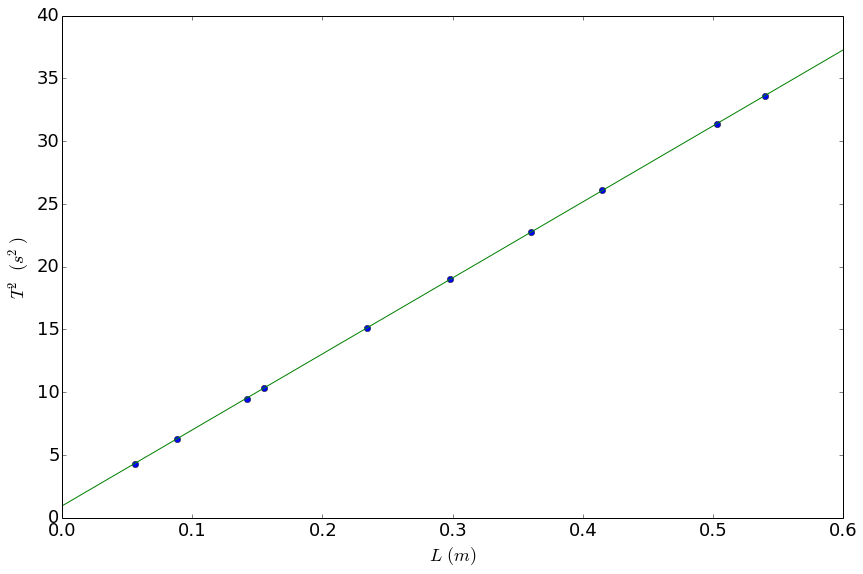
\includegraphics[scale=0.6]{graf1.png}
\caption{Gráfico da regressão linear de $T^2$ por $L$, sobreposta aos pontos obtidos experimentalmente.} 
\end{figure} 
\subsubsection{Estudo do coeficiente linear}

A interpretação física do coeficiente linear $a$ é 
$$ a = \frac{8\pi I_0}{G r^4}  $$
isolando G, obtemos:

$$ G = \frac{8\pi I_0}{a r^4}  $$
sendo que $r = d/2$, $\Delta r = {\Delta d}/{2} $. Logo,

 % substituir os dados reais %
$$ G = 21500414874914.6 \pi I $$

$$ \Delta G = \sqrt{\frac{64 \pi^{2} {\Delta I_0}^{2}}{a^{2} r^{8}} + \frac{64 \pi^{2} {\Delta a}^{2} {I_0}^{2}}{a^{4} r^{8}} + \frac{256 \pi^{2} {\Delta r}^{2} {I_0}^{2}}{a^{2} r^{10}}} $$


$$ = \sqrt{2841357013360.82 \pi^{2} {\Delta I}^{2} + 3624637429.80694 \pi^{2} I^{2}}$$







\section{Conclusões}



\end{document}
